%class
\documentclass[a4paper, 12pt]{article}

%encoding
\usepackage[T1]{fontenc}           %font encoding
\usepackage[utf8]{inputenc}         %script encoding

%packages
\usepackage[czech]{babel}           %language
\usepackage[a4paper, text={17cm,24cm}, left=2cm, top=3 cm]{geometry}		%layout
\usepackage{times}					%font
\usepackage[ruled, czech, linesnumbered, longend, noline]{algorithm2e}		%algorithms
\usepackage[unicode,hidelinks]{hyperref}	%links
\usepackage{amsmath}
\usepackage{tabularx}
\usepackage{multicol}
\usepackage{multirow}
\usepackage{graphicx}
\usepackage{float}
\usepackage{csquotes}
\usepackage{xcolor}
\usepackage{caption}
\usepackage{fixltx2e} % allow superscript and subscript in headings

\urlstyle{same}

\newcommand{\urlhref}[2]{\href{#1}{\textcolor{cyan}{\underline{#2}}}}
\newcommand{\iic}{I\textsuperscript{2}C }

\begin{document}

\begin{titlepage}
	\centering

	
\includegraphics{src/fitlogo.pdf}

	\vspace{\stretch{0.382}}

	{\Huge IMP projekt 2023\\[0.4em]
		\LARGE Meteostanice}

	\vspace{\stretch{0.618}}

	\begin{table}[H]
		\hfill
		\begin{tabularx}{0.3\textwidth}{Xr}
			David Tobolík & xtobol06 \\
		\end{tabularx}
	\end{table}
\end{titlepage}

\tableofcontents
\newpage

\section{Úvod}
Cílem projektu je vypracovat měření teploty a~vlhkosti senzorem SHT31 a~zobrazovat naměřené informace na displeji SSD1306, veškerá logika je řízena mikrokontrolerem ESP32. K~vypracování řešení bylo zvoleno prostředí idf\footnote{\url{https://github.com/espressif/esp-idf}}.

Výsledné řešení po spuštění volitelně přehraje animaci a~začne periodicky zobrazovat údaje o~teplotě a~vlhkosti, společně s~grafem naměřených hodnot. Graf i~zobrazená hodnota se aktualizují vždy před zobrazením příslušných údajů. Frekvence přepínání obrazovek je konfigurovatelná před sestavením aplikace a~ovlivňuje tedy i~frekvenci zaznamenávání dat do grafu.

\begin{figure}[H]
    \centering
    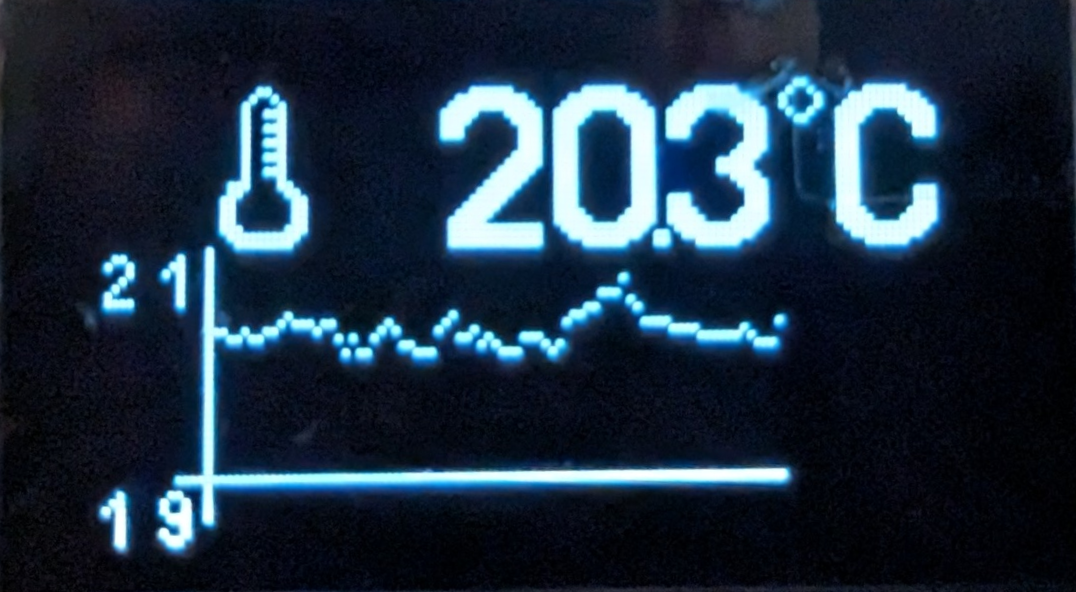
\includegraphics{src/temp.png} \\
    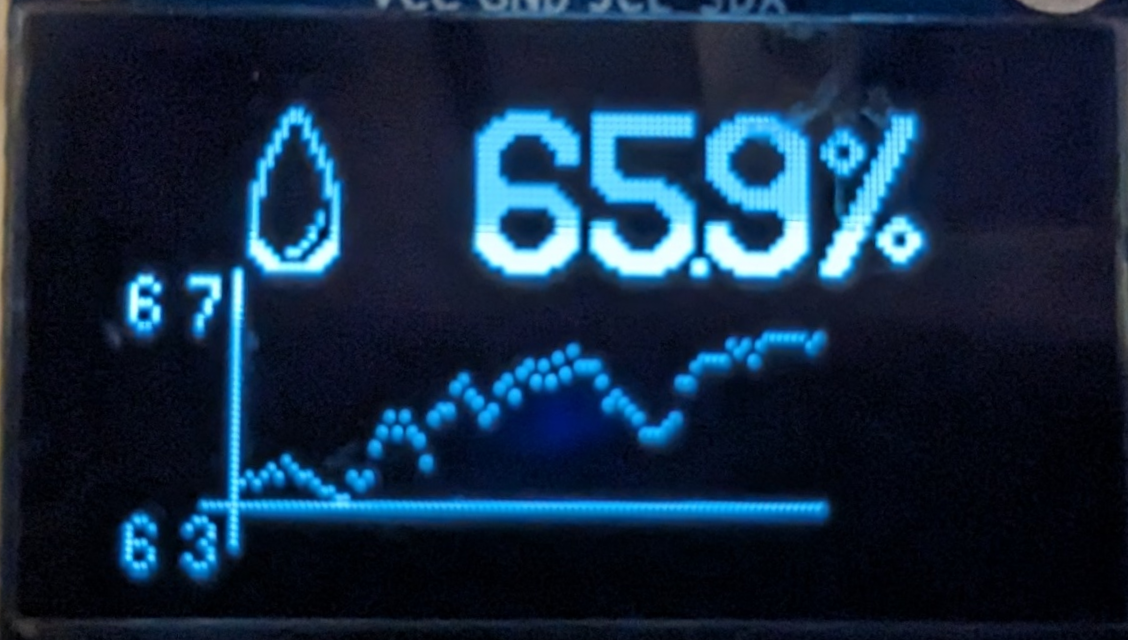
\includegraphics{src/humi.png}
    \caption{Ukázka naměřených hodnot s~intervalem měření 2 minuty}
\end{figure}

\newpage
\section{Schéma zapojení}
Schéma obsahuje výchozí čísla pinů, která lze změnit, viz sekce \ref{config}.
    \begin{figure}[H]
        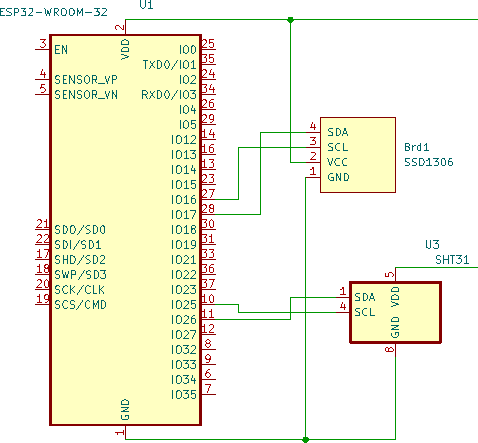
\includegraphics{src/schematic.pdf}
        \caption{Schéma zapojení\\ pozn. vcc v~tomto případě odpovídá 3v3 vcc}
    \end{figure}

\section{Konfigurace}\label{config}
Konfigurace programu probíhá před sestavením přes vestavěné rozhraní \texttt{menuconfig}. Lze povolit nebo zakázat úvodní animaci, nastavit periodu přepínání obrazovek s~teplotou a~vlhkostí a~nastavit konfiguraci jednotlivých periferií, konkrétně čísla GPIO pinů a~pracovní frekvenci. Všechna nastavení jsou dostupná z~hlavní strany pod \texttt{IMP project configuration}.

\section[Senzor SHT31]{Senzor SHT31\protect\footnote{\url{https://www.laskakit.cz/user/related\_files/sht3x.pdf}}}
Senzor SHT31 pro měření teploty a~vlhkosti podporuje režim jednorázového a~periodického měření, pro projekt byl využit pouze jednorázový režim. Měření v~tomto případě probíhá tak, že mcu zašle 2-bytový příkaz, který specifikuje, že se jedná o~jednorázové měření a~parametr opakovatelnosti měření (viz dokumentace k~senzoru), počká požadovanou dobu (dle zvolené opakovatelnosti) a~přečte data z~\iic rozhraní. Formát odpovědi je 6 bytů, postupně 2 byty hodnoty teploty, kontrolní byte pro teplotu, 2 byty hodnoty vlhkosti a~kontrolní byte pro vlhkost. Obě hodnoty jsou ve floating point formátu.

Získané hodnoty je potřeba zkontrolovat pomocí crc\footnote{\url{https://en.wikipedia.org/wiki/Cyclic\_redundancy\_check}} a~přepočíst na finální hodnotu teploty a~vlhkosti podle vzorce z~dokumentace.

\section[Displej SSD1306]{Displej SSD1306\protect\footnote{\url{https://www.laskakit.cz/user/related\_files/ssd1306.pdf}}}\label{ssd1306}
Pro řešení projektu je použito pouze rozhraní pro zapisování dat přes \iic do displeje, avšak displej podporuje i~mód čtení, především pro zjištění stavu paměti, který ale nebyl potřeba.

Zapisování dat probíhá ve 2 režimech\,--\,pro zasílání příkazů a~dat, z~nichž každý má variantu pro jeden byte nebo nepřetržitý tok dat. Řešení projektu používá pouze variantu pro tok dat (stream). Režim je určen prvním bytem (nepočítáme byte s~adresou a~režimem \iic) a~zbytek už je určen pro data nebo příkazy (toto platí pouze pro stream varianty).

Příkazy (commands) slouží především ke konfiguraci a~ovládání displeje. V~projektu jsou použity pro inicializaci displeje, avšak je možné posílat příkazy za běhu a~tím měnit např. režimy zobrazení, adresu, na kterou se zapisují data apod. Inicializace využívá sekvenci příkazů popsanou v~dokumentaci (Application note) s~několika úpravami. Nejdůležitější z~nich je nastavení horizontálního adresovacího režimu paměti, který zajistí správné namapování bufferu s~daty do RAM paměti displeje díky automatické inkrementaci čítače zapisované adresy, která se zalamuje na konci řádků displeje.

Data určují, co bude zobrazeno na displeji. Displej má 128x64 pixelů a~je rozdělen na strany\,--\,strana obsahuje 8 pixelů na výšku, displej má tedy dohromady 8 stran a~každá strana obsahuje 128 sloupců po 8 pixelech. Data jsou uložena ve struktuře \texttt{display\_buff}, která odpovídá osmi polím/stranám po 128 bytech.

\section{Implementace}
Implementace je v~jazyce C pouze s~využitím základních knihoven a~driveru k~\iic rozhraní\footnote{\url{https://docs.espressif.com/projects/esp-idf/en/latest/esp32/api-reference/peripherals/i2c.html}}. Veškeré ovládání periferií je implementováno pouze s~využitím tohoto rozhraní. V~následujících sekcích je postupně popsány jednotlivé kroky programu.

    \subsection{Inicializace \iic rozhraní}
    Pro práci se zařízeními je použita struktura \texttt{dev\_conf\_t}, která obsahuje \iic adresu a~port, frekvenci hodinového signálu a~čísla pinů pro hodinový signál a~datový tok. Inicializace probíhá ve funkci \texttt{i2c\_init()}, která nastaví potřebné hodnoty a~zavolá funkci pro instalaci \iic driveru.

    \subsection{Měření teploty a~vlhkosti}
    Hlavní smyčka programu volá funkci pro měření a~zobrazení teploty, poté počká zvolenou dobu, zavolá funkci pro měření a~zobrazení vlhkosti, opět počká a~celá smyčka se opakuje.

    Zobrazení veškerých znaků je řešeno zápisem dat z~hlavičkového souboru \texttt{glyphs.h} do bufferu, který je nejprve naplněn daty a~poté poslán přes \iic rozhraní do displeje jako data (viz sekce \ref{ssd1306}). Slouží k~tomu především funkce \texttt{write\_to\_buff()}, která na danou stranu a~x-ovou souřadnici zapíše data o~dané šířce a~výšce. Šířka je v~jednotkách, které odpovídají jednomu sloupci dat/pixelů na straně displeje, výška udává počet stran, které se mají zapsat. Jednotlivé glyfy jsou uloženy jako surová data, která odpovídají jejich zobrazení na displeji, tedy LSB odpovídá prvnímu pixelu na dané straně a~MSB tomu poslednímu. Všechny glyfy jsou vlastnoručně vytvořené pomocí přiložené tabulky \href{run:../glyph-maker.ods}{\texttt{glyph-maker.ods}}.

    Měření probíhá ve funkci \texttt{sht31\_get\_data()}, která změří data výše popsaným způsobem a~vrací strukturu s~naměřenou teplotou a~vlhkostí. Data se přidají do dat grafu, případně se aktualizuje maximální a~minimální hodnota naměřených dat.

    \subsection{Ukládání naměřených hodnot do grafu}
    Struktura dat grafu si ukládá současný index, minimální a~maximální hodnotu a~informaci o~tom, jestli došlo k~naplnění maximálního počtu dat grafu, který je specifikován v~souboru \texttt{utils.h} pod \texttt{MAX\_GRAPH\_DATA}.

    Dokud není struktura plná, data se dále přidávají dokud nedojde k~naplnění struktury a~přitom se aktualizuje maximum a~minimum, v~tomto případě stačí porovnat novou hodnotu se stávajícím minimem a~maximem. Když dojde k~naplnění struktury, nastaví se příznak naplnění a~při dalším přidání hodnoty do grafu je potřeba naměřená data posunout (zahodí se nejstarší hodnota a~přidá se nová). Pro vypočítání nového maxima a~minima je nutné projít všechna data, protože minimum a~maximum už nemusí být aktuální.

    \subsection{Zobrazování naměřených dat v~grafu}
    Zápis dat grafu do bufferu provádí funkce \texttt{draw\_graph()}. Základní je zjištění rozsahu hodnot dat pro zobrazení, které odpovídá $|\lceil v_{max}\rceil - \lfloor v_{min} \rfloor|$, pokud předpokládáme, že $v$ jsou naměřené hodnoty. Pokud by měl být rozsah příliš malý (stanoveno hodnotou \texttt{GRAPH\_DATA\_MIN\_RANGE}) nastaví se na minimální rozsah. Podle zvoleného rozsahu dat se dopočítají hranice rozsahu zaokrouhlené na celá čísla.

    Zvolené hranice se zapíší do bufferu vedle os grafu a~začnou se mapovat a~zapisovat jednotlivá data. Data se mapují tak, aby nejnižší bod grafu odpovídal zvolené spodní hranici a~nejvyšší bod grafu zase zvolené horní hranici. Pro každou hodnotu je nutné vypočítat vzdálenost v~pixelech od spodní hranice, v~tomto případě dochází k~přepočítávání x a~y souřadnic na strany a~nastavuje se konkrétní pixel ve sloupci strany. Mapování probíhá podle následujícího vzorce

    $$ (v_i - lower\_bound) * \frac{GRAPH\_POINT\_MAX\_RANGE}{data\_range}$$

    \subsection{Zobrazení dat na displej}
    V~tento moment už jsou v~bufferu zapsána všechna data pro vykreslení a~celý buffer se jako data pošle přes \iic rozhraní displeji, viz sekce \ref{ssd1306}.

\end{document}

